\documentclass[11pt,a4paper]{article}

\usepackage[utf8]{inputenc}
\usepackage[T1]{fontenc}
\usepackage[french]{babel}
\usepackage{lmodern}
\usepackage{amsmath}
\usepackage{amssymb}
\usepackage{graphicx}
\usepackage{booktabs}
\usepackage{geometry}
\usepackage{float}
\usepackage{subcaption}
\geometry{margin=2.5cm}
\graphicspath{{figures/}{figures/gap_tests/}}

\title{Étude statistique des décimales de $\pi$ et construction d'un générateur uniforme}
\author{}
\date{}

\begin{document}

\maketitle

\section{Introduction}

L'objectif de ce projet est d'étudier expérimentalement si les décimales de $\pi$ présentent des propriétés compatibles avec celles d'une suite pseudo-aléatoire. L'étude porte d'abord directement sur les chiffres décimaux de $\pi$, puis sur un générateur uniforme construit à partir de ces chiffres.

Le générateur proposé reste volontairement simple : les décimales sont découpées en blocs non chevauchants de taille $k$, chaque bloc est interprété comme un entier, puis normalisé par division par $10^k$ afin d'obtenir une valeur dans $[0,1[$. Les valeurs obtenues sont ensuite comparées aux valeurs produites par \texttt{random.random()} de Python.

Les tests utilisés sont le test du $\chi^2$, le test de Kolmogorov--Smirnov et le gap test. Dans tout le rapport, le seuil de décision est fixé à $5\%$. Une p-value faible conduit à rejeter l'hypothèse nulle au seuil choisi ; une p-value élevée signifie seulement que les observations sont compatibles avec cette hypothèse, et non que l'hypothèse est démontrée.

\section{Rappels théoriques}

\subsection{Test du $\chi^2$}

Le test du $\chi^2$ compare des effectifs observés $O_i$ à des effectifs attendus $E_i$. La statistique utilisée est
\[
\chi^2 = \sum_{i=1}^{r} \frac{(O_i-E_i)^2}{E_i}.
\]
Dans ce projet, il est utilisé de deux manières : sur les chiffres $0,\ldots,9$ des décimales de $\pi$, puis sur des classes de même largeur de l'intervalle $[0,1[$ pour les générateurs.

\subsection{Test de Kolmogorov--Smirnov}

Le test de Kolmogorov--Smirnov compare la fonction de répartition empirique $F_n$ à la fonction de répartition théorique $F$. Sa statistique est
\[
D_n = \sup_x |F_n(x)-F(x)|.
\]
Pour une loi uniforme sur $[0,1[$, on a $F(x)=x$ sur cet intervalle. Ce test est adapté aux variables continues. Il est donc pertinent pour les valeurs générées dans $[0,1[$, mais moins adapté lorsque $k$ est très petit, car les valeurs possibles sont alors très discrètes.

\subsection{Gap test}

Le gap test étudie les longueurs des écarts entre deux occurrences successives d'un événement. Si l'événement a une probabilité $p$ et si les observations sont indépendantes, la longueur $G$ d'un écart suit le modèle
\[
P(G=m)=p(1-p)^m.
\]
Pour les chiffres de $\pi$, l'événement est l'apparition d'un chiffre cible, avec $p=0{,}1$. Pour les générateurs dans $[0,1[$, l'événement retenu dans le code est
\[
0{,}2 \leq U < 0{,}3,
\]
ce qui donne également $p=0{,}1$. Les écarts de longueur supérieure ou égale à 18 sont regroupés dans une dernière classe afin d'obtenir des effectifs suffisants.

\section{Étude directe des décimales de $\pi$}

\subsection{Données utilisées}

Le script lit le fichier contenant les décimales de $\pi$, supprime les caractères non numériques et retire le premier chiffre 3 afin de ne conserver que les décimales. L'étude est réalisée sur $1\,000\,000$ décimales.

\subsection{Uniformité des chiffres}

L'hypothèse nulle du test du $\chi^2$ est que les dix chiffres $0,\ldots,9$ apparaissent avec la même probabilité. Les résultats sont donnés dans le tableau \ref{tab:digits_chi2}.

\begin{table}[H]
\centering
\begin{tabular}{lcc}
\toprule
Test & Statistique & p-value \\
\midrule
$\chi^2$ sur les chiffres & 5.509080 & 0.787867 \\
\bottomrule
\end{tabular}
\caption{Test du $\chi^2$ sur les fréquences des décimales de $\pi$.}
\label{tab:digits_chi2}
\end{table}

Au seuil de $5\%$, on ne rejette pas $H_0$. Les fréquences observées sont donc compatibles avec une répartition uniforme des chiffres.

\begin{figure}[H]
\centering
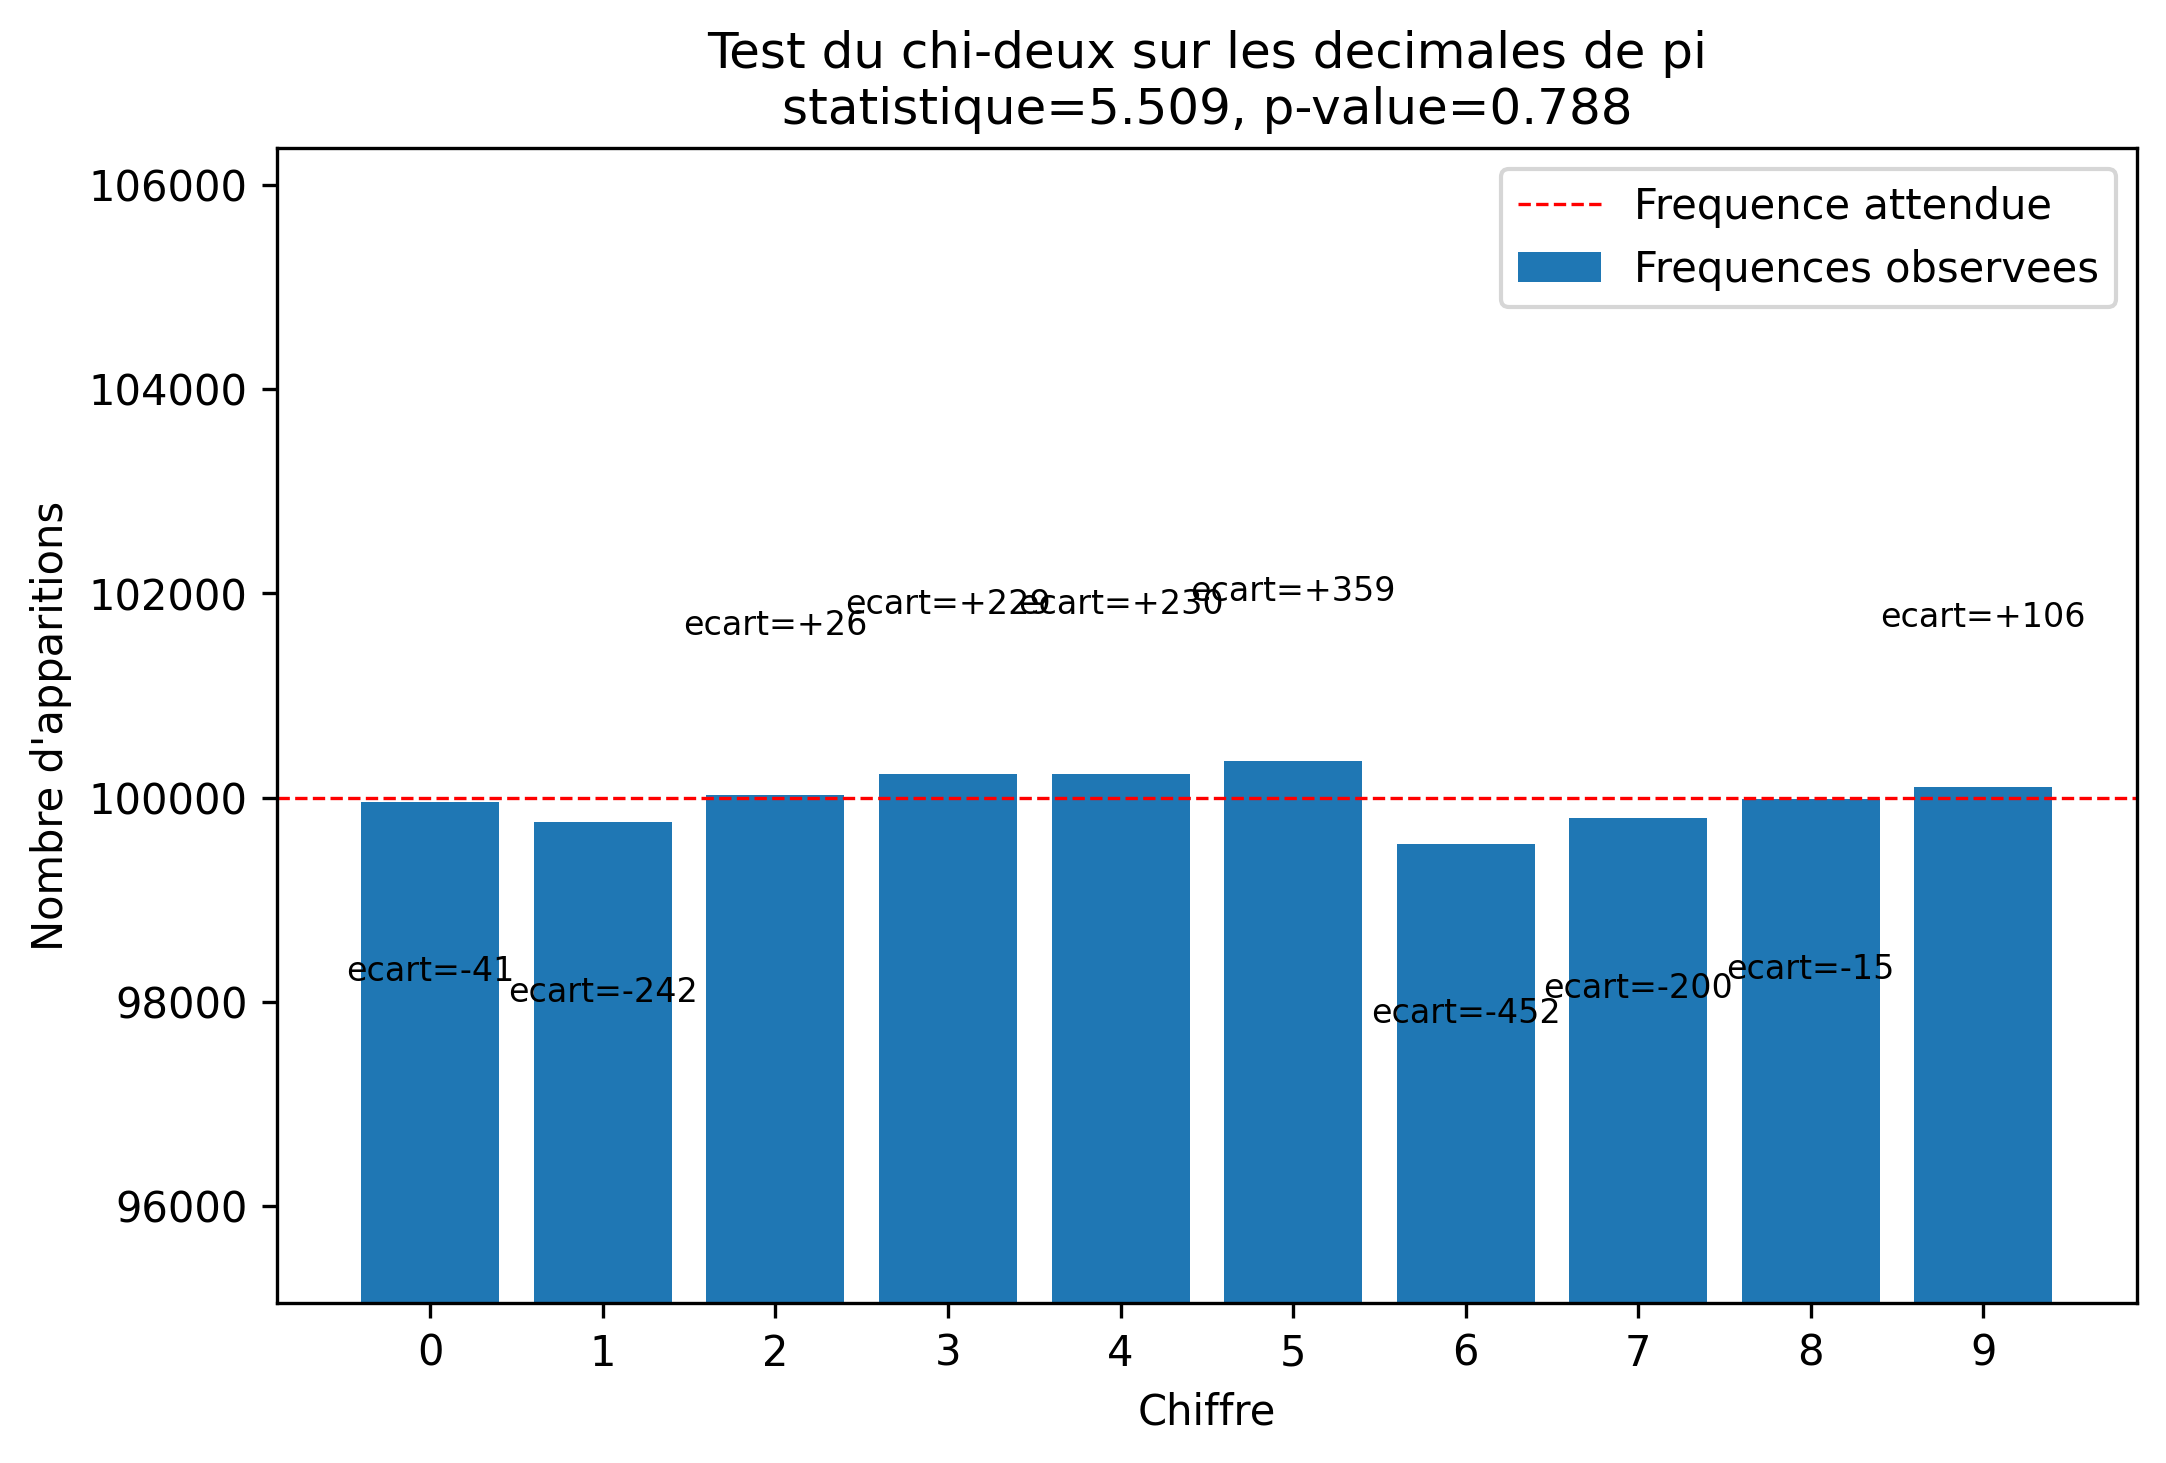
\includegraphics[width=0.78\textwidth]{chi_squared.png}
\caption{Fréquences observées des chiffres de $\pi$ et fréquence attendue sous uniformité.}
\label{fig:chi_squared_digits}
\end{figure}

\subsection{Gap test sur les chiffres}

Le gap test est appliqué à chacun des dix chiffres cibles. Le tableau \ref{tab:gap_digits} résume les p-values obtenues.

\begin{table}[H]
\centering
\begin{tabular}{cccc}
\toprule
Chiffre cible & Statistique & p-value & Conclusion au seuil de 5\% \\
\midrule
0 & 14.700177 & 0.682441 & On ne rejette pas $H_0$ \\
1 & 23.184593 & 0.183596 & On ne rejette pas $H_0$ \\
2 & 16.180691 & 0.579938 & On ne rejette pas $H_0$ \\
3 & 6.055168 & 0.995968 & On ne rejette pas $H_0$ \\
4 & 31.183954 & 0.027408 & On rejette $H_0$ \\
5 & 18.317082 & 0.434955 & On ne rejette pas $H_0$ \\
6 & 11.365508 & 0.878208 & On ne rejette pas $H_0$ \\
7 & 14.763216 & 0.678156 & On ne rejette pas $H_0$ \\
8 & 16.384735 & 0.565716 & On ne rejette pas $H_0$ \\
9 & 25.550316 & 0.110493 & On ne rejette pas $H_0$ \\
\bottomrule
\end{tabular}
\caption{Gap test appliqué aux dix chiffres cibles.}
\label{tab:gap_digits}
\end{table}

Pour le chiffre 7, utilisé comme exemple détaillé dans la sortie du programme, on ne rejette pas $H_0$. La figure \ref{fig:gap_target_7} montre la comparaison entre les effectifs observés et les effectifs attendus.

\begin{figure}[H]
\centering
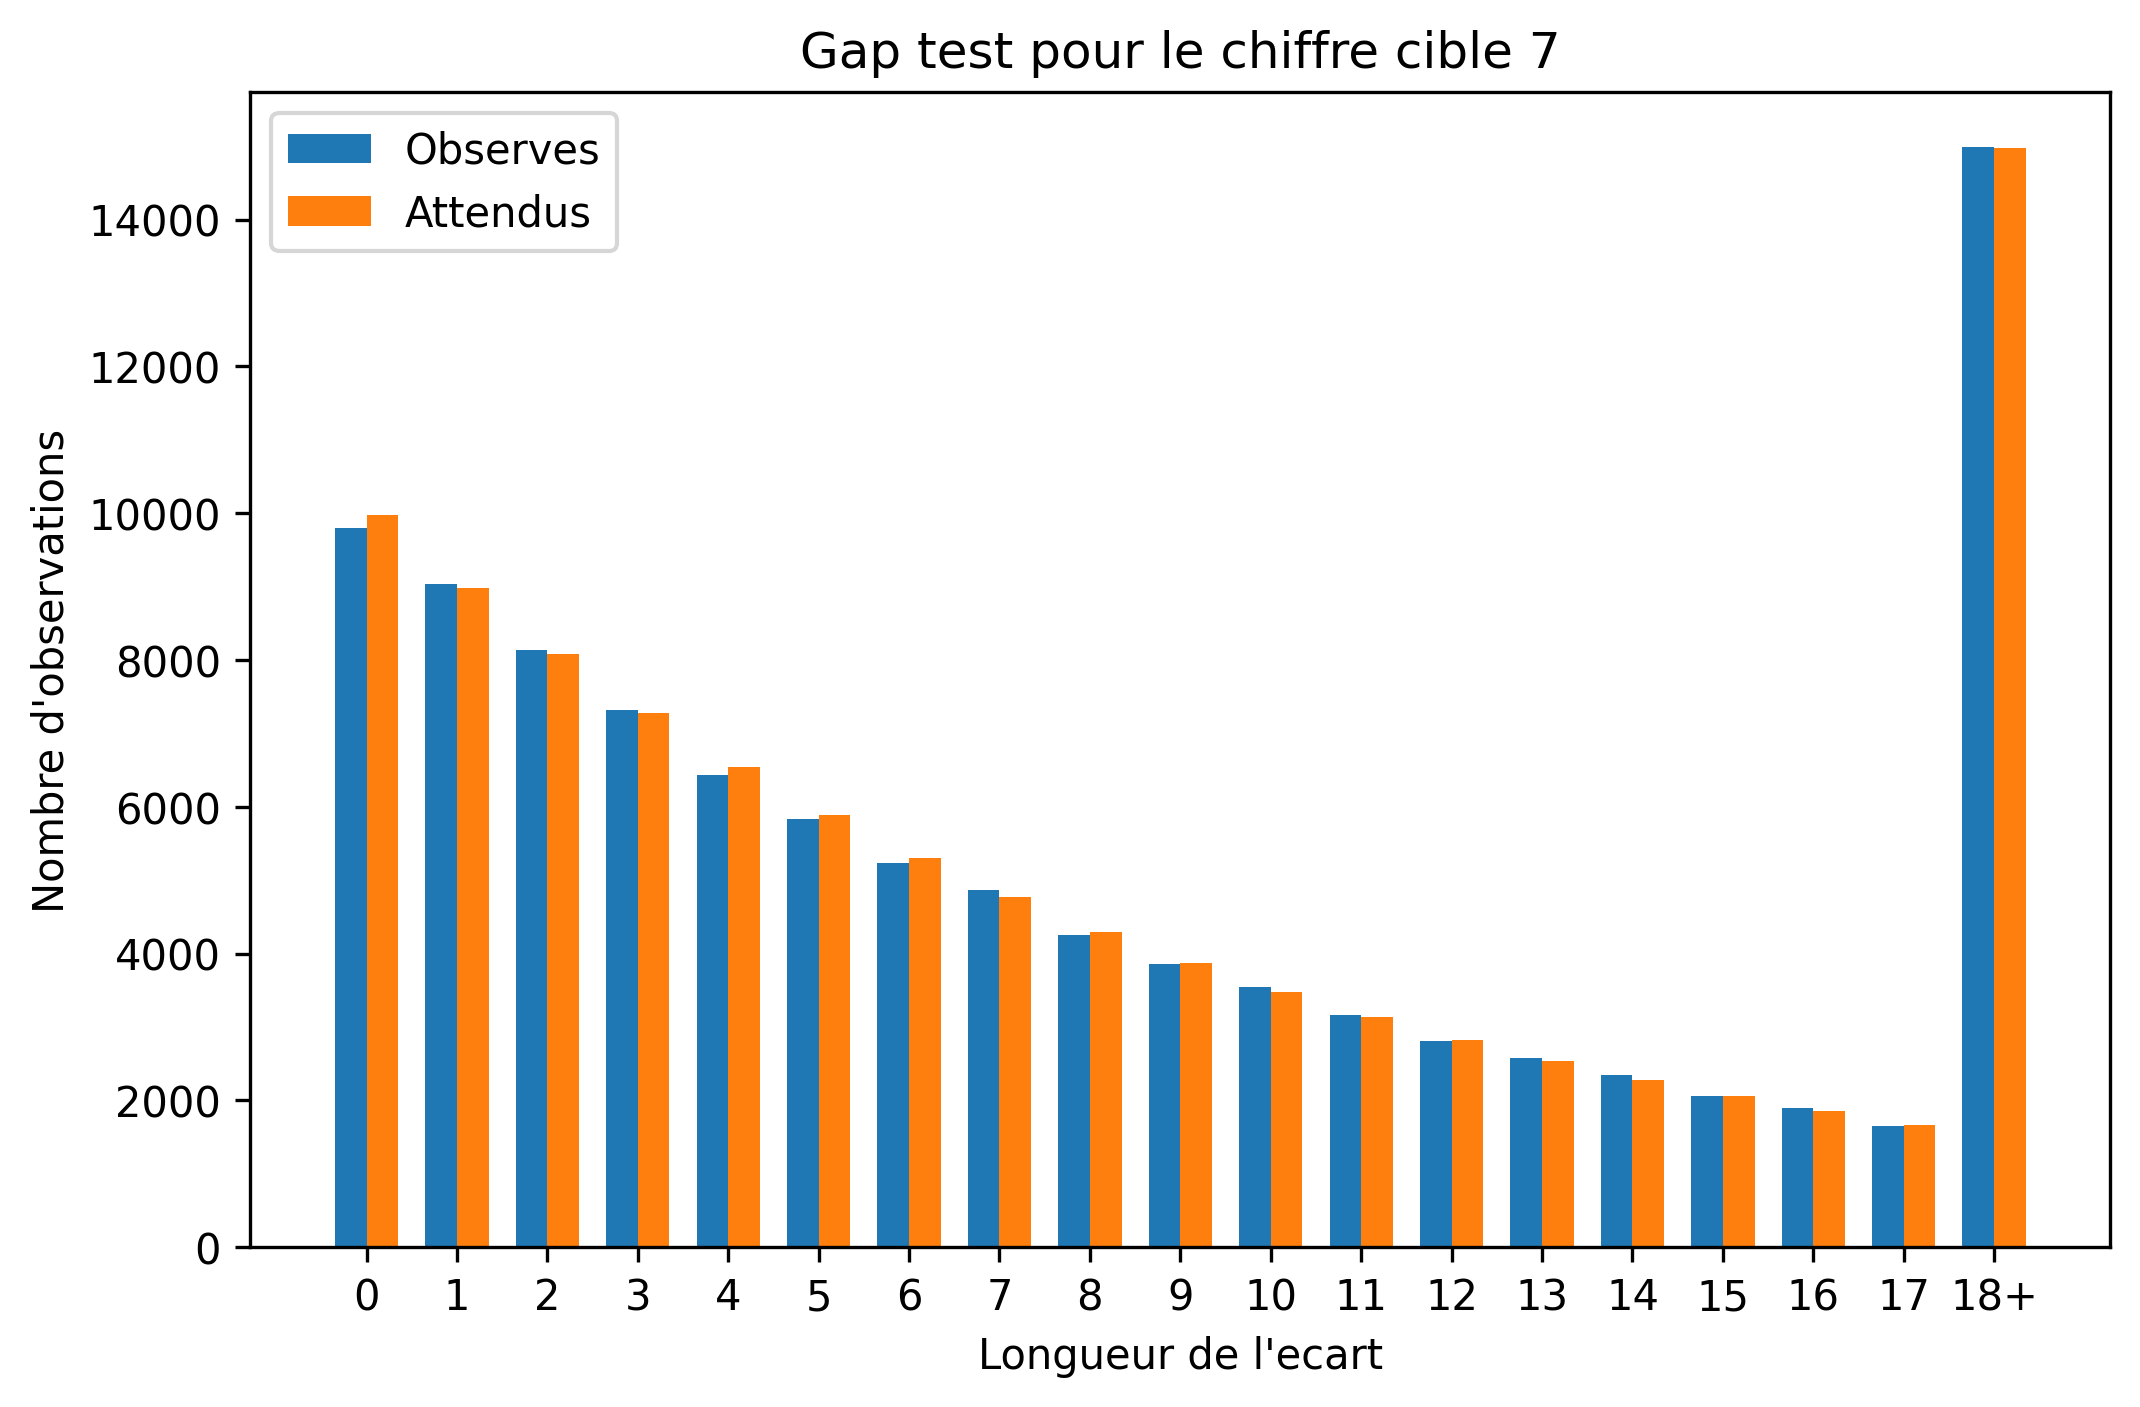
\includegraphics[width=0.78\textwidth]{gap_target_7.png}
\caption{Gap test pour le chiffre cible 7.}
\label{fig:gap_target_7}
\end{figure}

Le seul rejet au seuil de $5\%$ concerne le chiffre 4. Cette observation doit être interprétée avec prudence. Dix tests sont effectués simultanément, un pour chaque chiffre cible ; dans ce contexte, obtenir occasionnellement une p-value inférieure à $5\%$ reste plausible. De plus, l'échantillon contient un million de décimales, ce qui rend les tests très sensibles à de faibles écarts. Ce résultat suggère donc une fluctuation détectable pour le chiffre 4, mais ne permet pas de conclure que les décimales de $\pi$ ne se comportent pas comme une suite pseudo-aléatoire.

\begin{figure}[H]
\centering
\begin{subfigure}{0.48\textwidth}
\centering
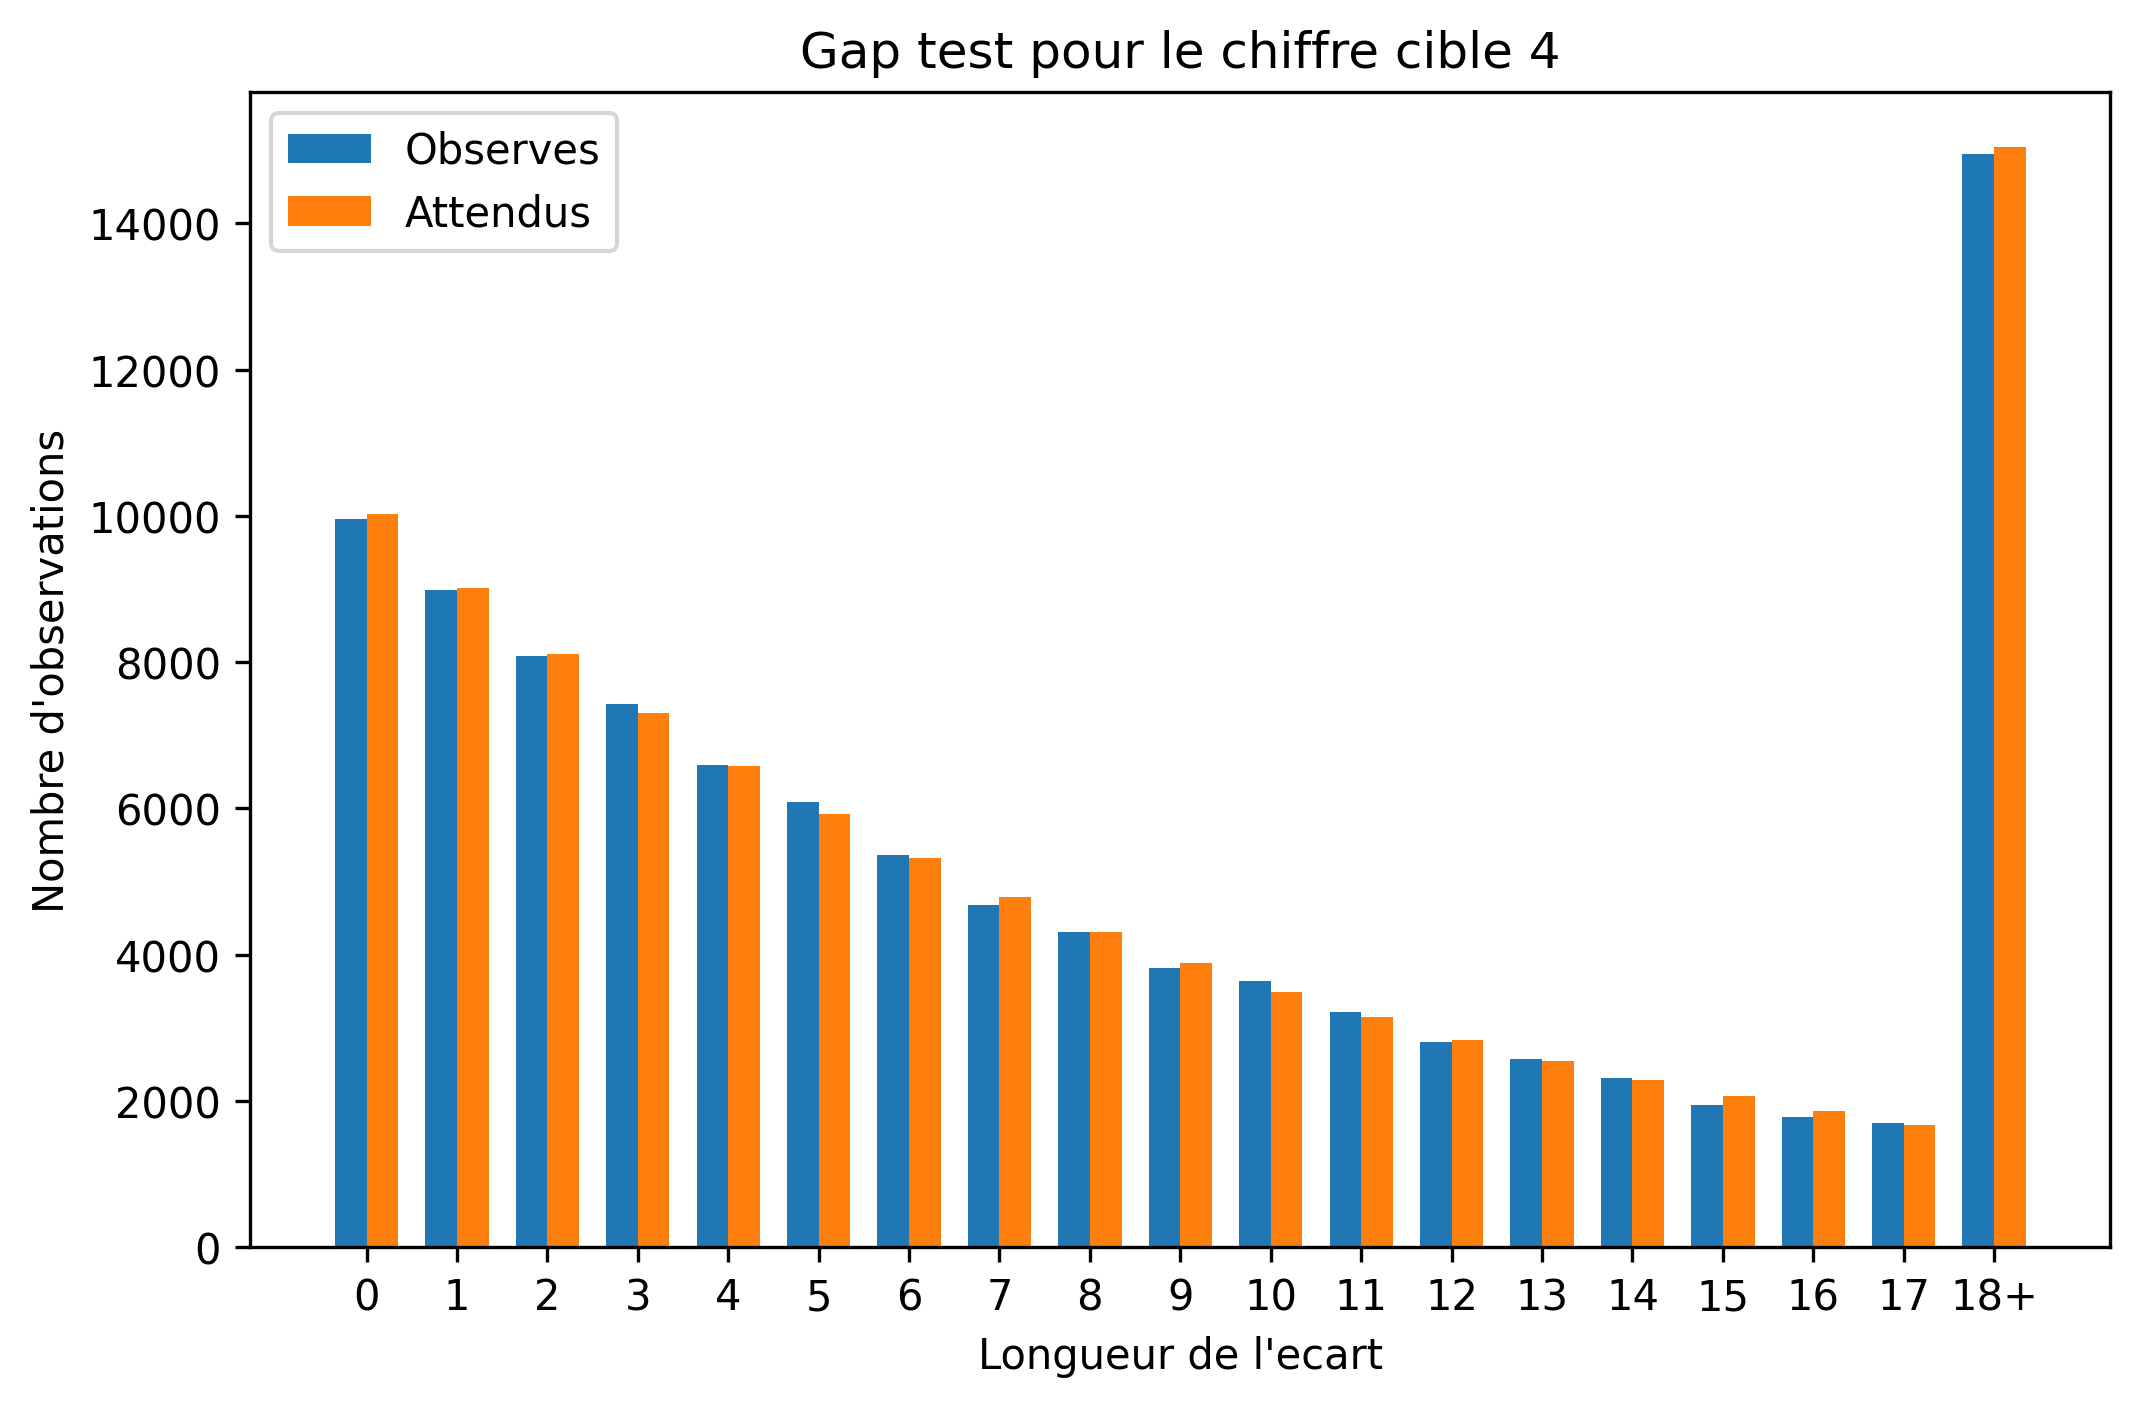
\includegraphics[width=\textwidth]{gap_target_4.png}
\caption{Chiffre cible 4.}
\label{fig:gap_target_4}
\end{subfigure}
\hfill
\begin{subfigure}{0.48\textwidth}
\centering
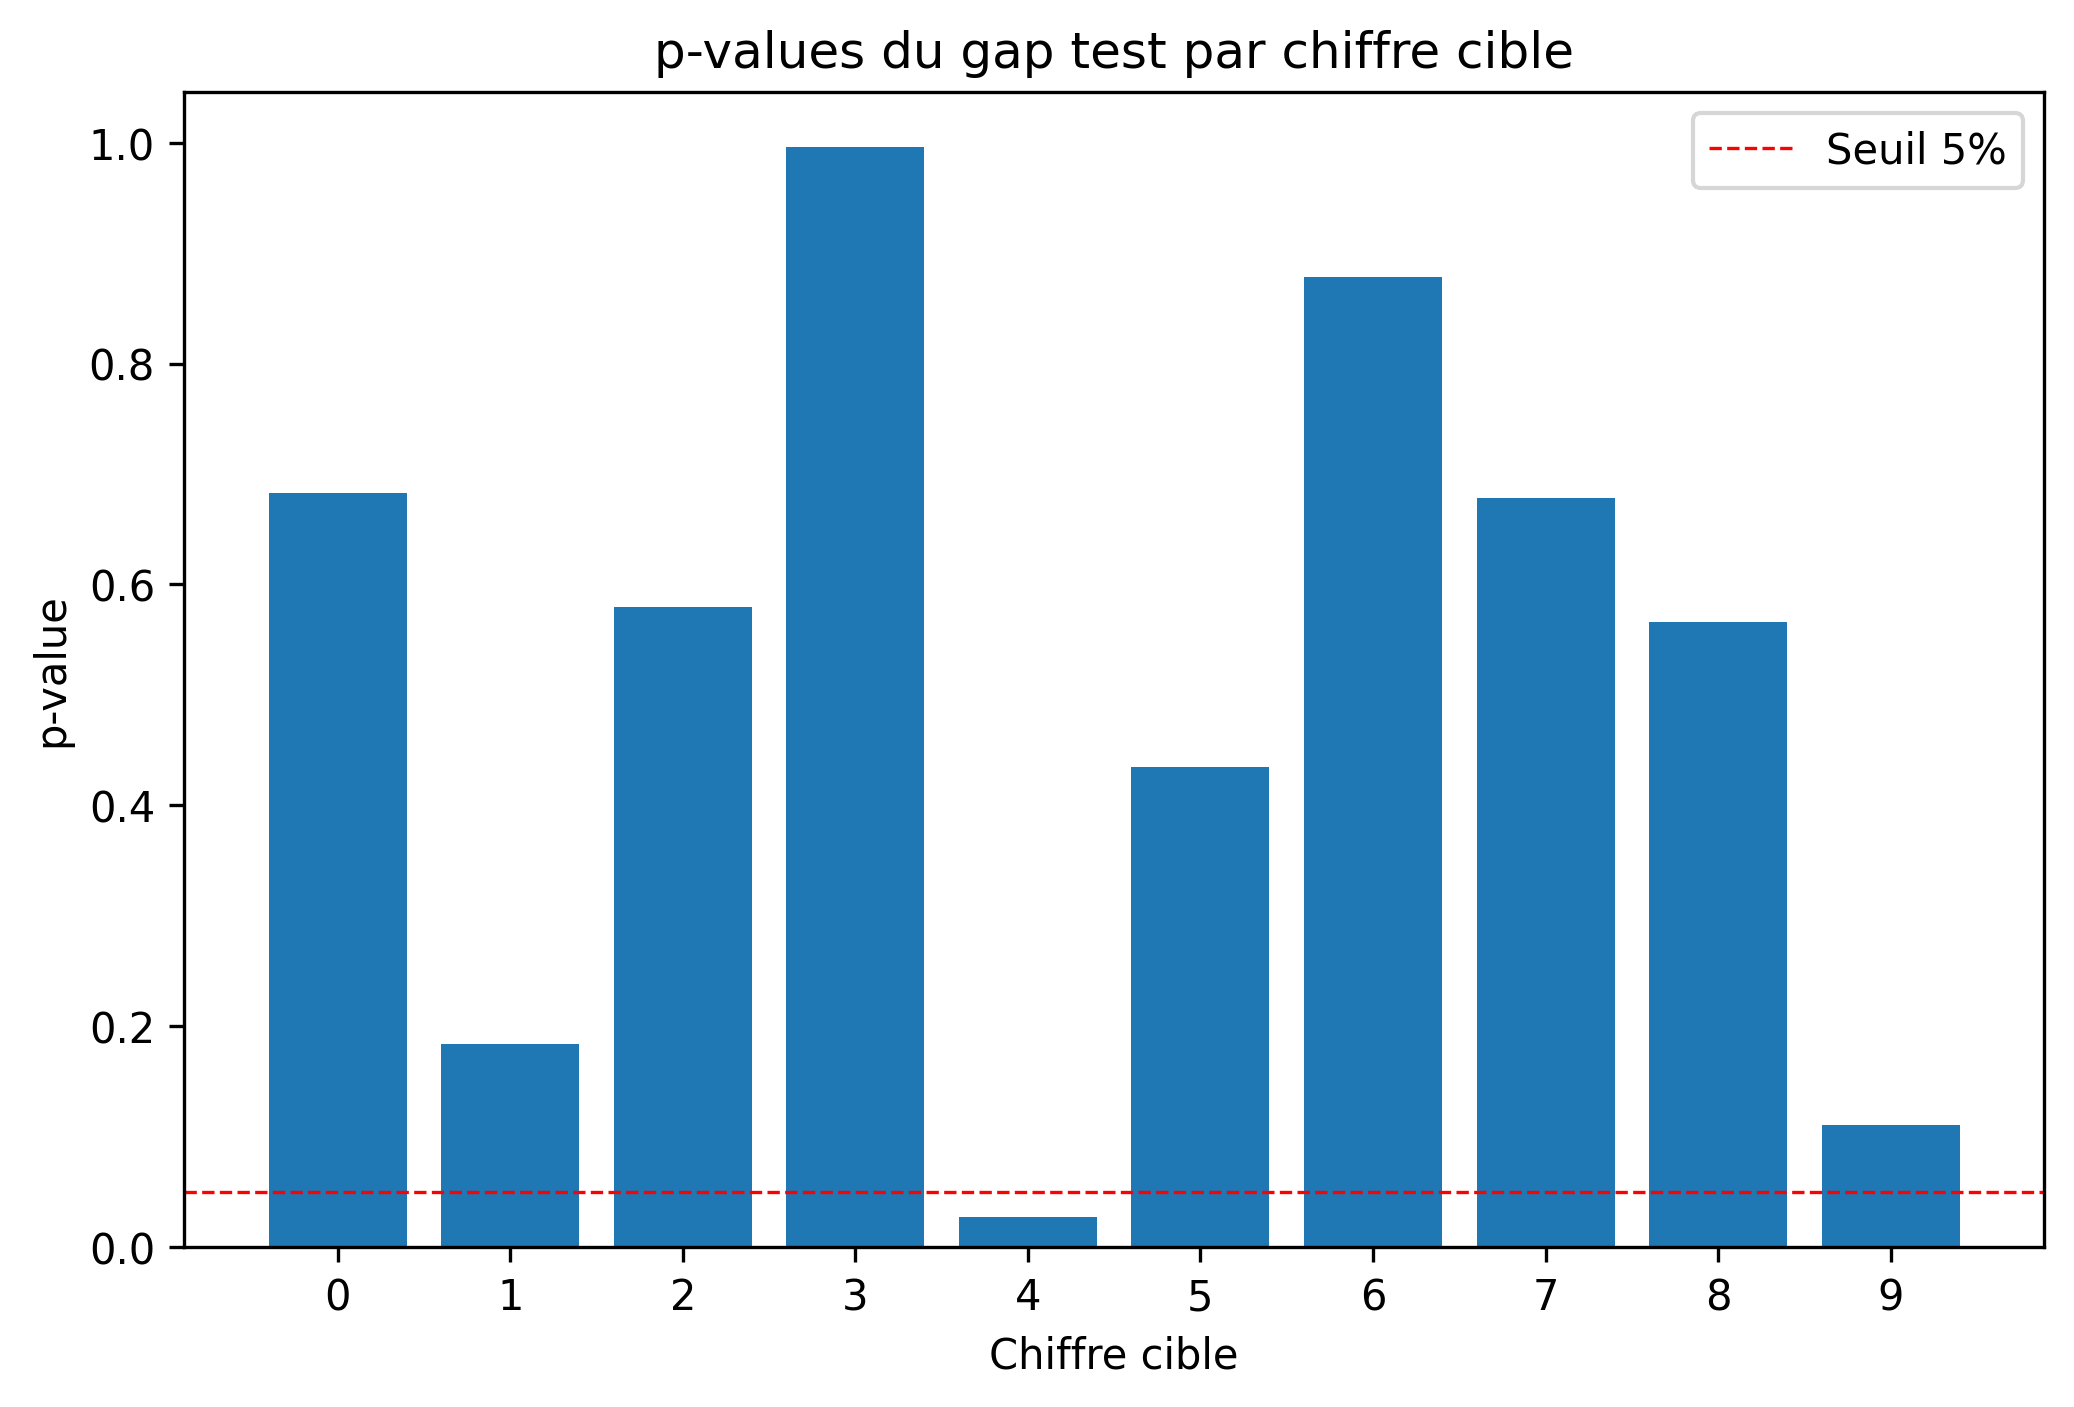
\includegraphics[width=\textwidth]{gap_pvalues_by_target.png}
\caption{p-values par chiffre cible.}
\label{fig:gap_pvalues}
\end{subfigure}
\caption{Synthèse du gap test sur les chiffres de $\pi$.}
\label{fig:gap_digits_summary}
\end{figure}

\section{Construction du générateur uniforme basé sur $\pi$}

\subsection{Définition du générateur}

Soit $k$ la taille d'un bloc. Les décimales de $\pi$ sont découpées en blocs non chevauchants :
\[
d_1d_2\ldots d_k,\quad d_{k+1}d_{k+2}\ldots d_{2k},\quad \ldots
\]
Chaque bloc est transformé en entier
\[
B_i = \sum_{j=1}^{k} d_{(i-1)k+j}10^{k-j},
\]
puis en nombre réel
\[
U_i = \frac{B_i}{10^k}.
\]
Ainsi, $U_i \in [0,1[$. Dans les comparaisons principales, le code utilise $k=6$, ce qui produit $166\,666$ valeurs à partir du million de décimales disponibles.

\subsection{Influence de la taille des blocs}

Le test de Kolmogorov--Smirnov est appliqué pour $k=1,\ldots,9$. Les résultats sont donnés dans le tableau \ref{tab:ks_by_k} et les figures \ref{fig:ks_by_k}.

\begin{table}[H]
\centering
\begin{tabular}{ccccc}
\toprule
$k$ & Nombre de valeurs & Statistique KS & p-value & Conclusion \\
\midrule
1 & 1\,000\,000 & 0.100561 & 0.000000 & On rejette $H_0$ \\
2 & 500\,000 & 0.011114 & 0.000000 & On rejette $H_0$ \\
3 & 333\,333 & 0.001319 & 0.607876 & On ne rejette pas $H_0$ \\
4 & 250\,000 & 0.001508 & 0.620132 & On ne rejette pas $H_0$ \\
5 & 200\,000 & 0.001645 & 0.650995 & On ne rejette pas $H_0$ \\
6 & 166\,666 & 0.001343 & 0.924527 & On ne rejette pas $H_0$ \\
7 & 142\,857 & 0.003969 & 0.022159 & On rejette $H_0$ \\
8 & 125\,000 & 0.001586 & 0.911604 & On ne rejette pas $H_0$ \\
9 & 111\,111 & 0.003106 & 0.233748 & On ne rejette pas $H_0$ \\
\bottomrule
\end{tabular}
\caption{Test de Kolmogorov--Smirnov pour différentes tailles de blocs.}
\label{tab:ks_by_k}
\end{table}

Pour $k=1$ et $k=2$, les valeurs générées ne peuvent prendre qu'un petit nombre de valeurs distinctes. La distribution est donc très discrète, ce qui explique que le test KS rejette nettement l'hypothèse d'uniformité continue. À partir de $k=3$, les résultats sont globalement compatibles avec une loi uniforme, même si $k=7$ donne une p-value inférieure à $5\%$. Le choix $k=6$ est un compromis simple : il produit suffisamment de valeurs tout en limitant l'effet de discrétisation.

\begin{figure}[H]
\centering
\begin{subfigure}{0.48\textwidth}
\centering
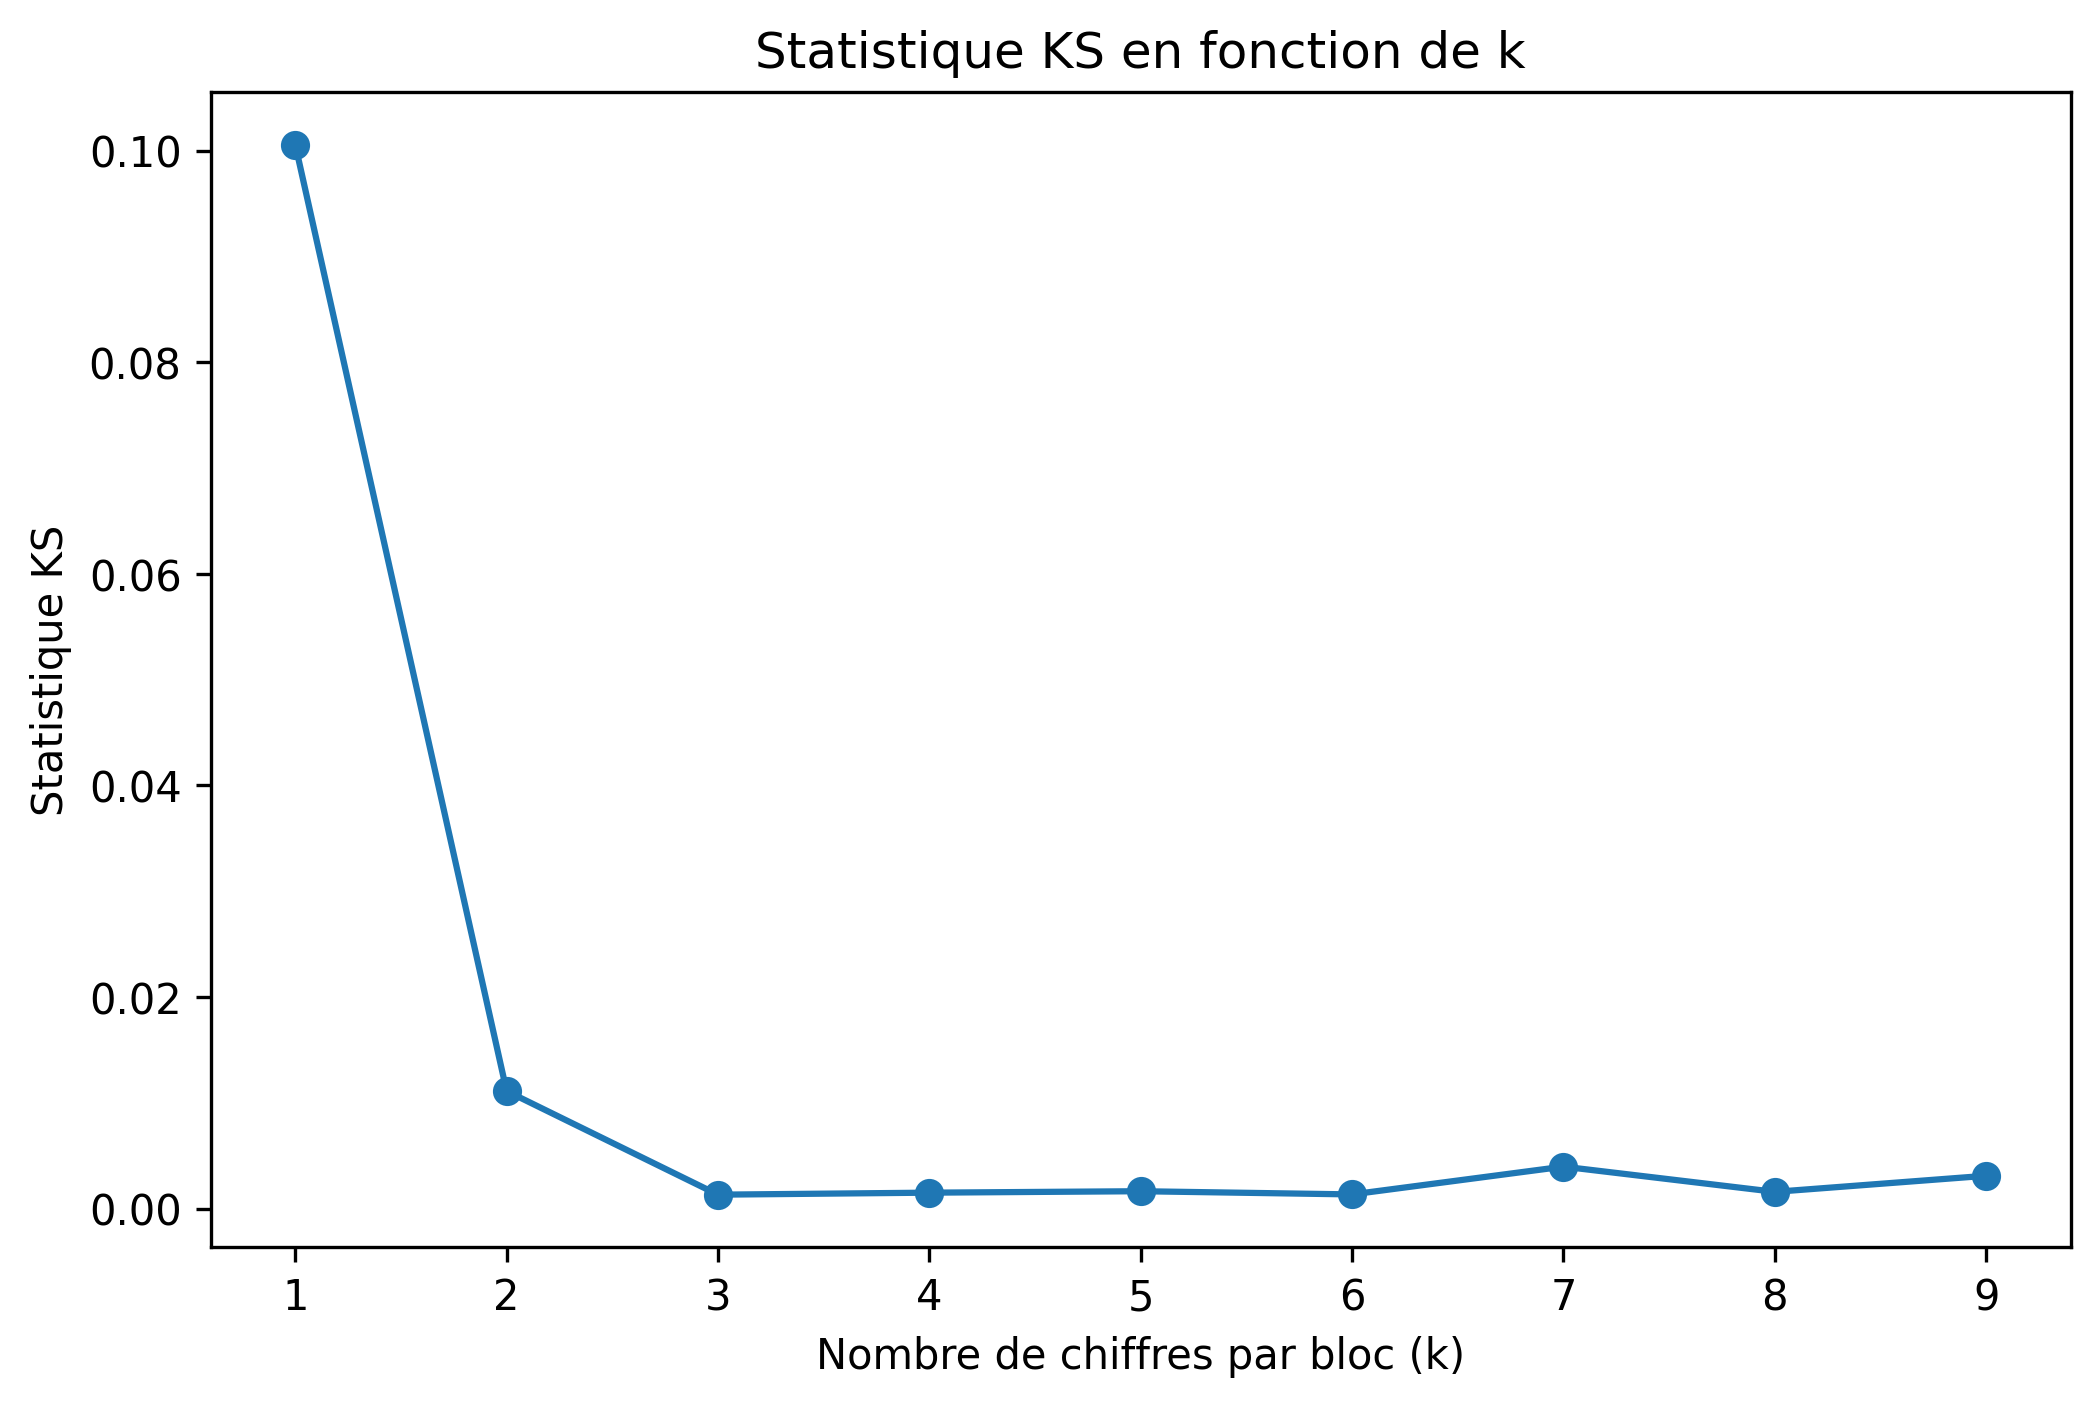
\includegraphics[width=\textwidth]{ks_statistic_by_k.png}
\caption{Statistique KS.}
\end{subfigure}
\hfill
\begin{subfigure}{0.48\textwidth}
\centering
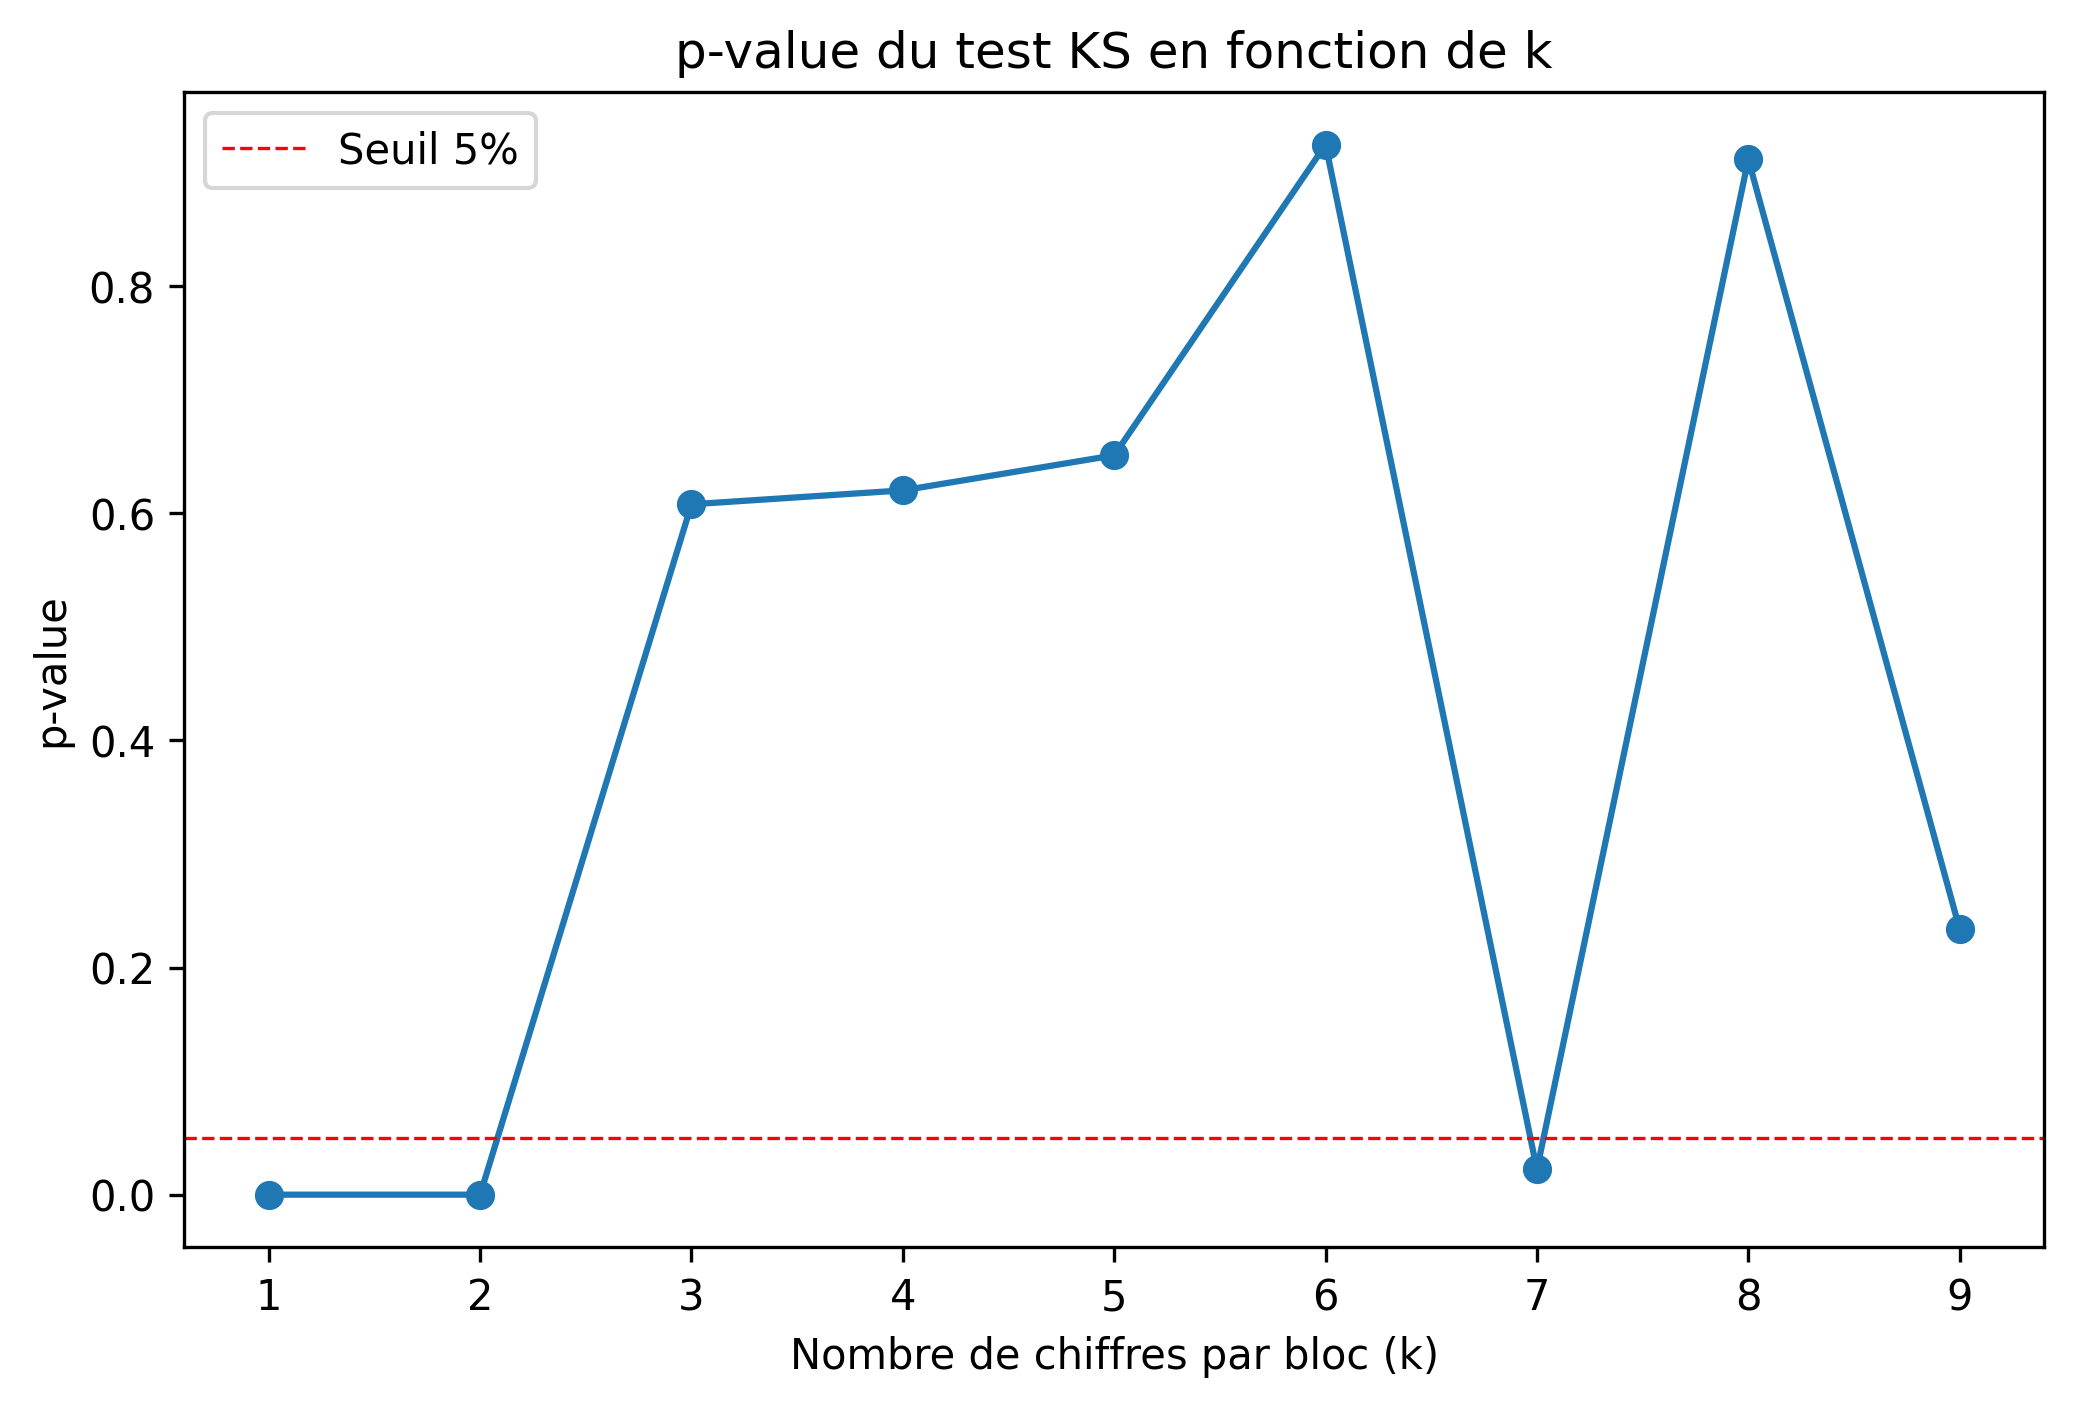
\includegraphics[width=\textwidth]{ks_pvalue_by_k.png}
\caption{p-values.}
\end{subfigure}
\caption{Influence de la taille des blocs sur le test KS du générateur basé sur $\pi$.}
\label{fig:ks_by_k}
\end{figure}

\section{Comparaison avec \texttt{random.random()} de Python}

Le générateur basé sur $\pi$ avec $k=6$ est comparé à \texttt{random.random()} de Python. Pour rendre la comparaison reproductible, le script fixe la graine de Python à 12345. Les deux générateurs produisent $166\,666$ valeurs.

\subsection{Tests appliqués aux deux générateurs}

Les mêmes tests sont appliqués aux deux suites de valeurs : test du $\chi^2$ sur dix classes de même largeur de $[0,1[$, test de Kolmogorov--Smirnov contre la loi uniforme sur $[0,1[$ et gap test sur l'événement $0{,}2 \leq U < 0{,}3$.

\begin{table}[H]
\centering
\begin{tabular}{llccc}
\toprule
Générateur & Test & Statistique & p-value & Conclusion au seuil de 5\% \\
\midrule
$\pi$, $k=6$ & $\chi^2$ sur classes & 5.138205 & 0.822098 & On ne rejette pas $H_0$ \\
$\pi$, $k=6$ & Kolmogorov--Smirnov & 0.001343 & 0.924527 & On ne rejette pas $H_0$ \\
$\pi$, $k=6$ & Gap test & 12.855109 & 0.800108 & On ne rejette pas $H_0$ \\
Python & $\chi^2$ sur classes & 9.987304 & 0.351514 & On ne rejette pas $H_0$ \\
Python & Kolmogorov--Smirnov & 0.003078 & 0.084929 & On ne rejette pas $H_0$ \\
Python & Gap test & 14.745893 & 0.679335 & On ne rejette pas $H_0$ \\
\bottomrule
\end{tabular}
\caption{Comparaison statistique du générateur basé sur $\pi$ et de \texttt{random.random()}.}
\label{tab:generator_comparison}
\end{table}

Pour les trois tests, les p-values obtenues sont supérieures à $5\%$ pour les deux générateurs. Les résultats sont donc compatibles avec l'hypothèse d'une loi uniforme sur $[0,1[$ et avec le modèle géométrique attendu pour les écarts de l'événement choisi.

\begin{figure}[H]
\centering
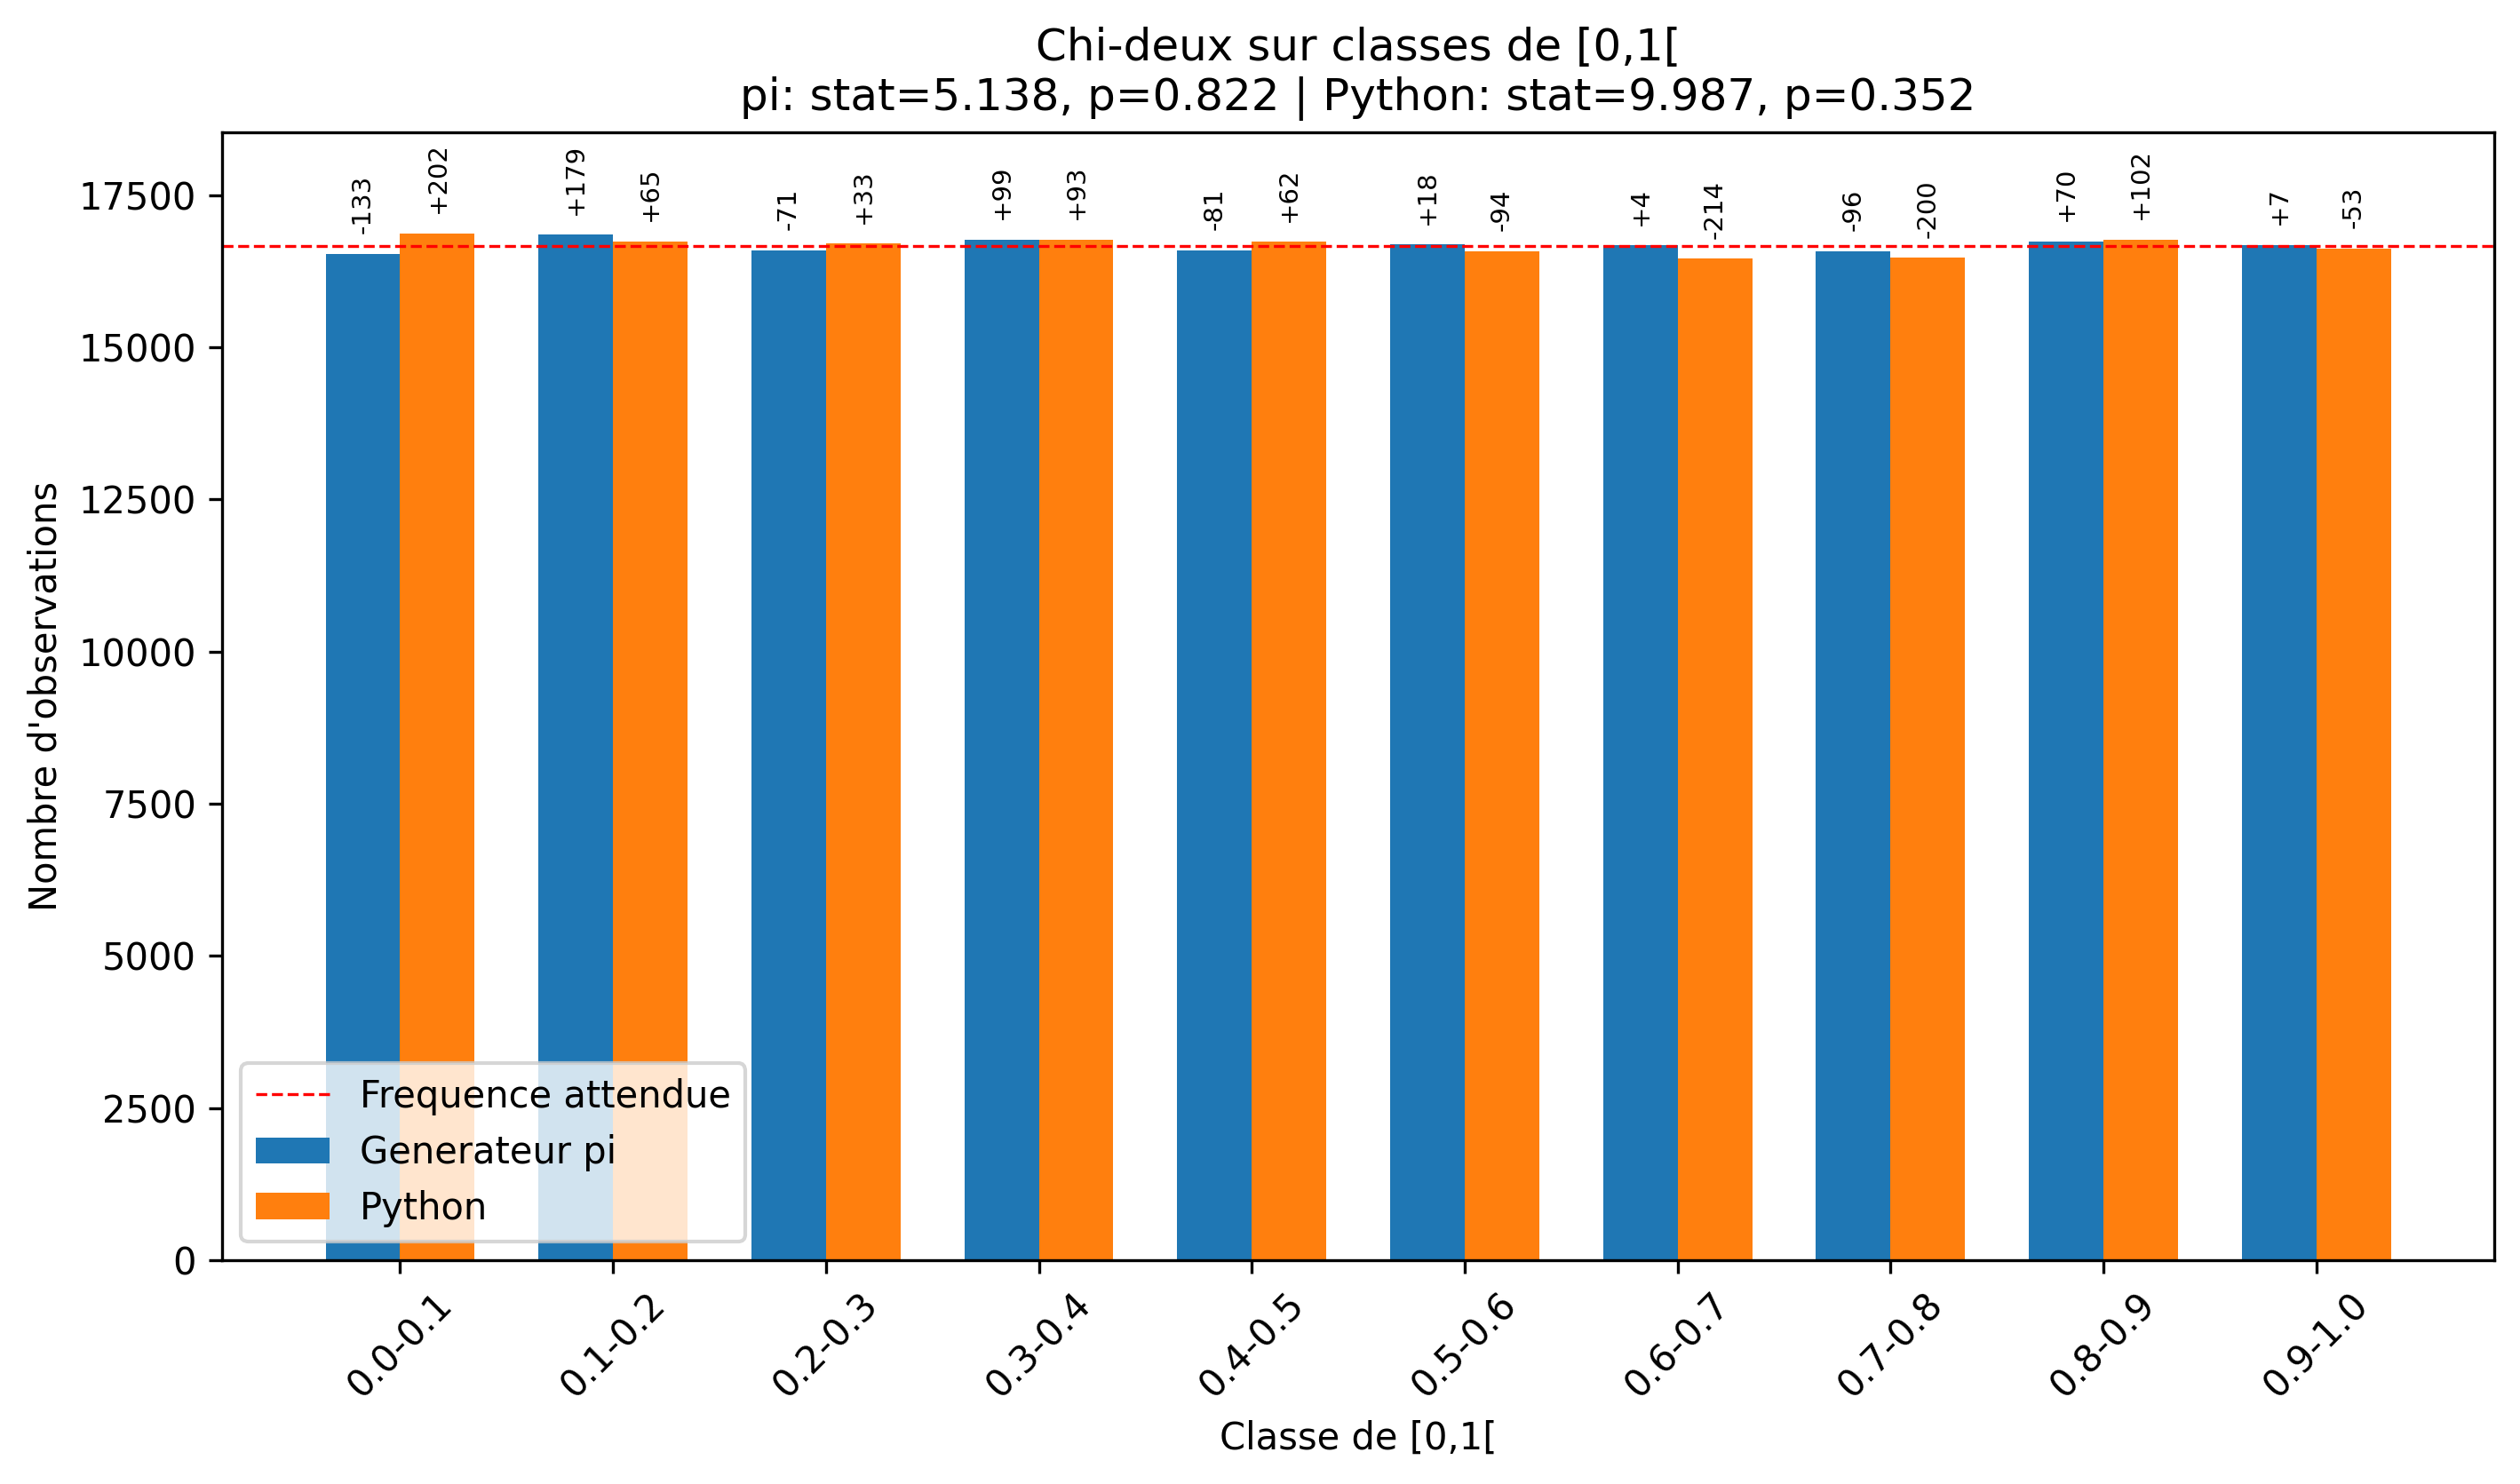
\includegraphics[width=0.9\textwidth]{comparison_chi_squared_uniform.png}
\caption{Comparaison des deux générateurs par test du $\chi^2$ sur dix classes de $[0,1[$.}
\label{fig:comparison_chi2}
\end{figure}

\begin{figure}[H]
\centering
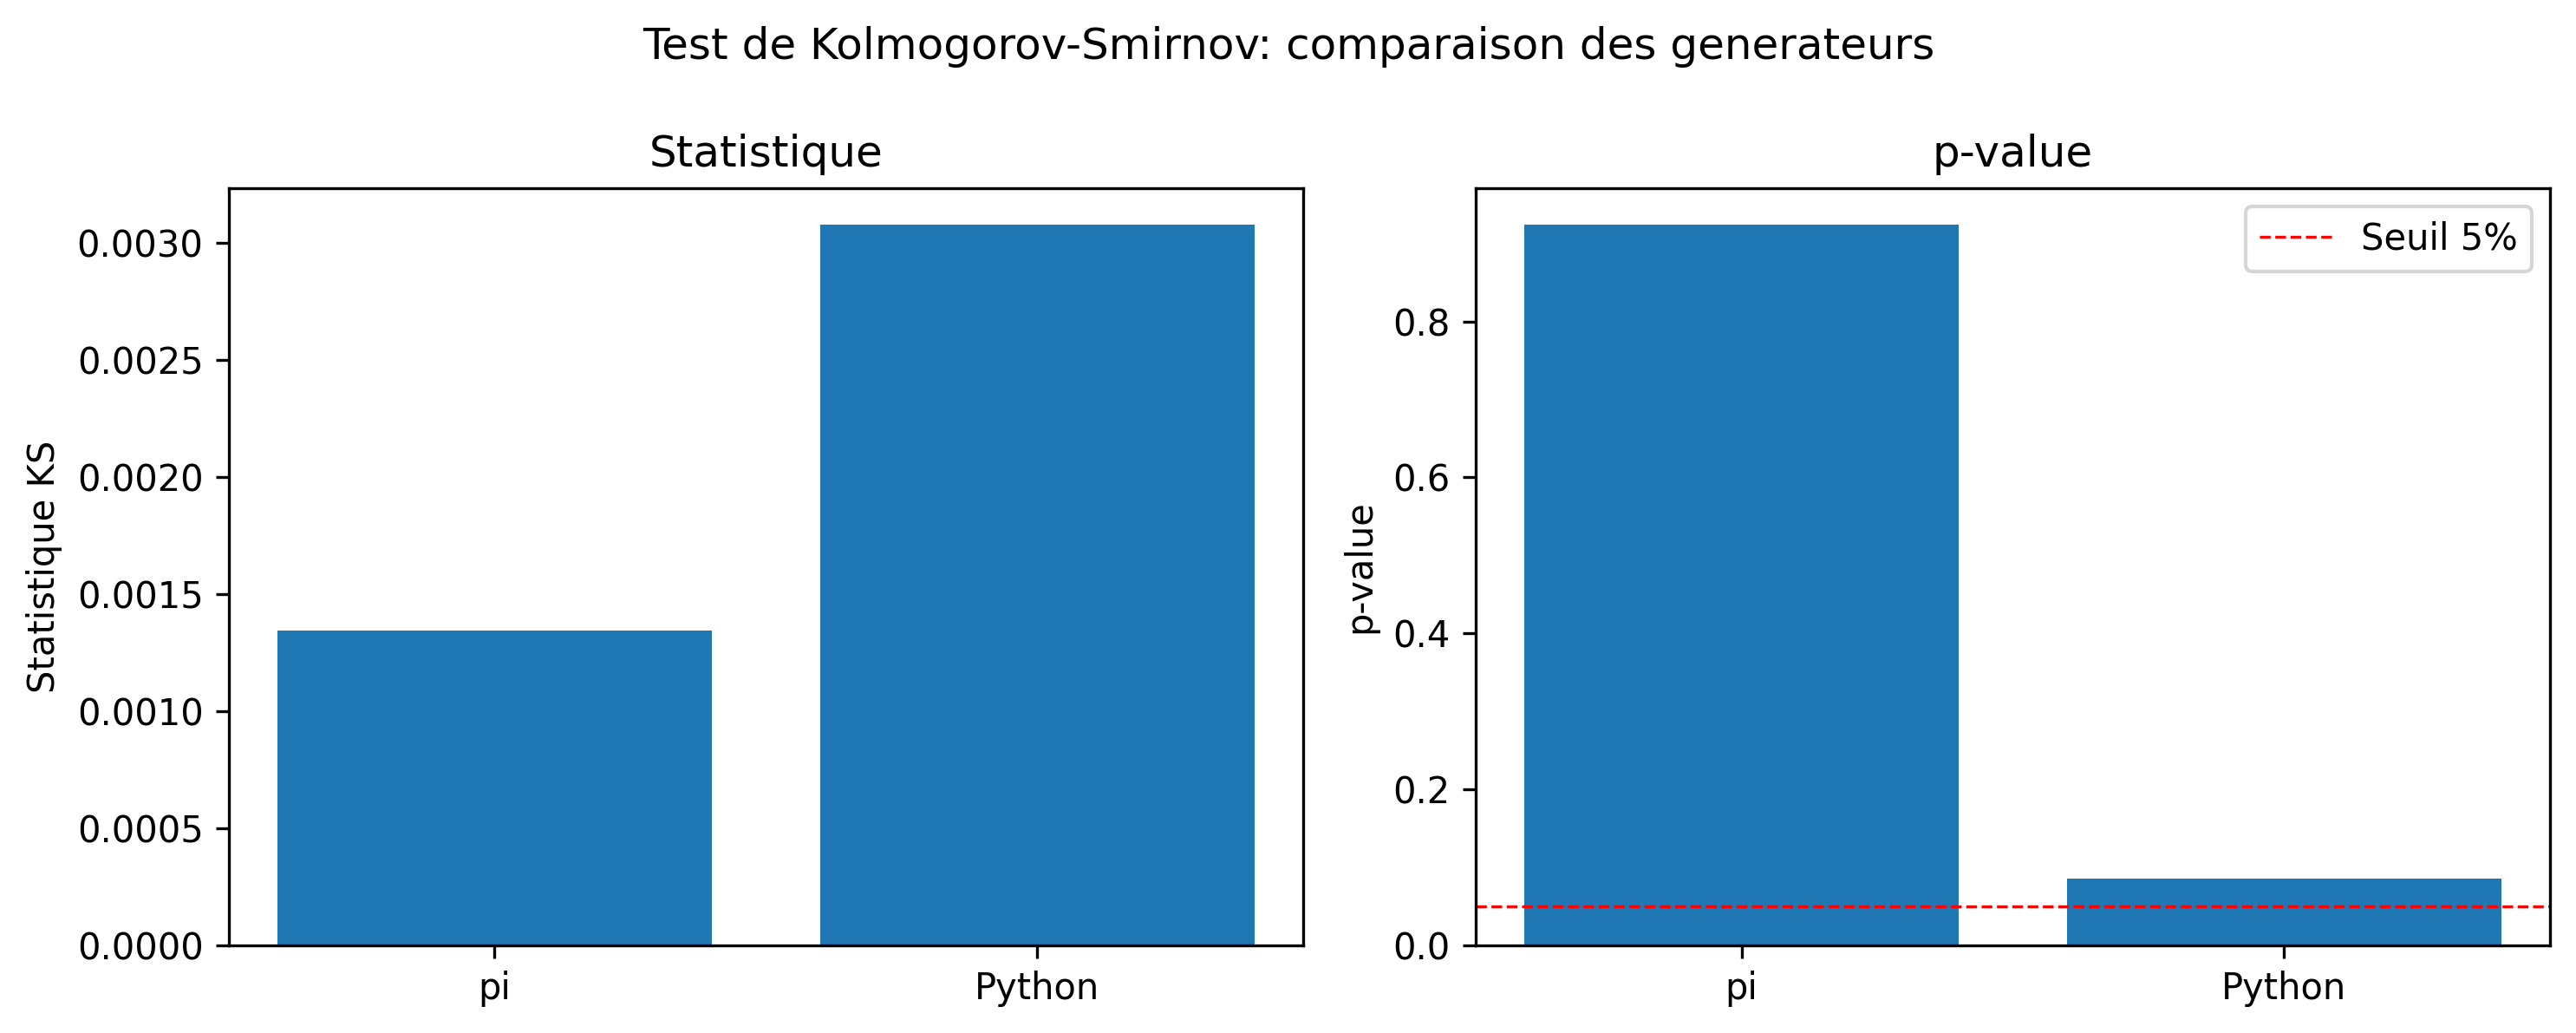
\includegraphics[width=0.9\textwidth]{comparison_ks_uniform.png}
\caption{Comparaison des deux générateurs par test de Kolmogorov--Smirnov.}
\label{fig:comparison_ks}
\end{figure}

\begin{figure}[H]
\centering
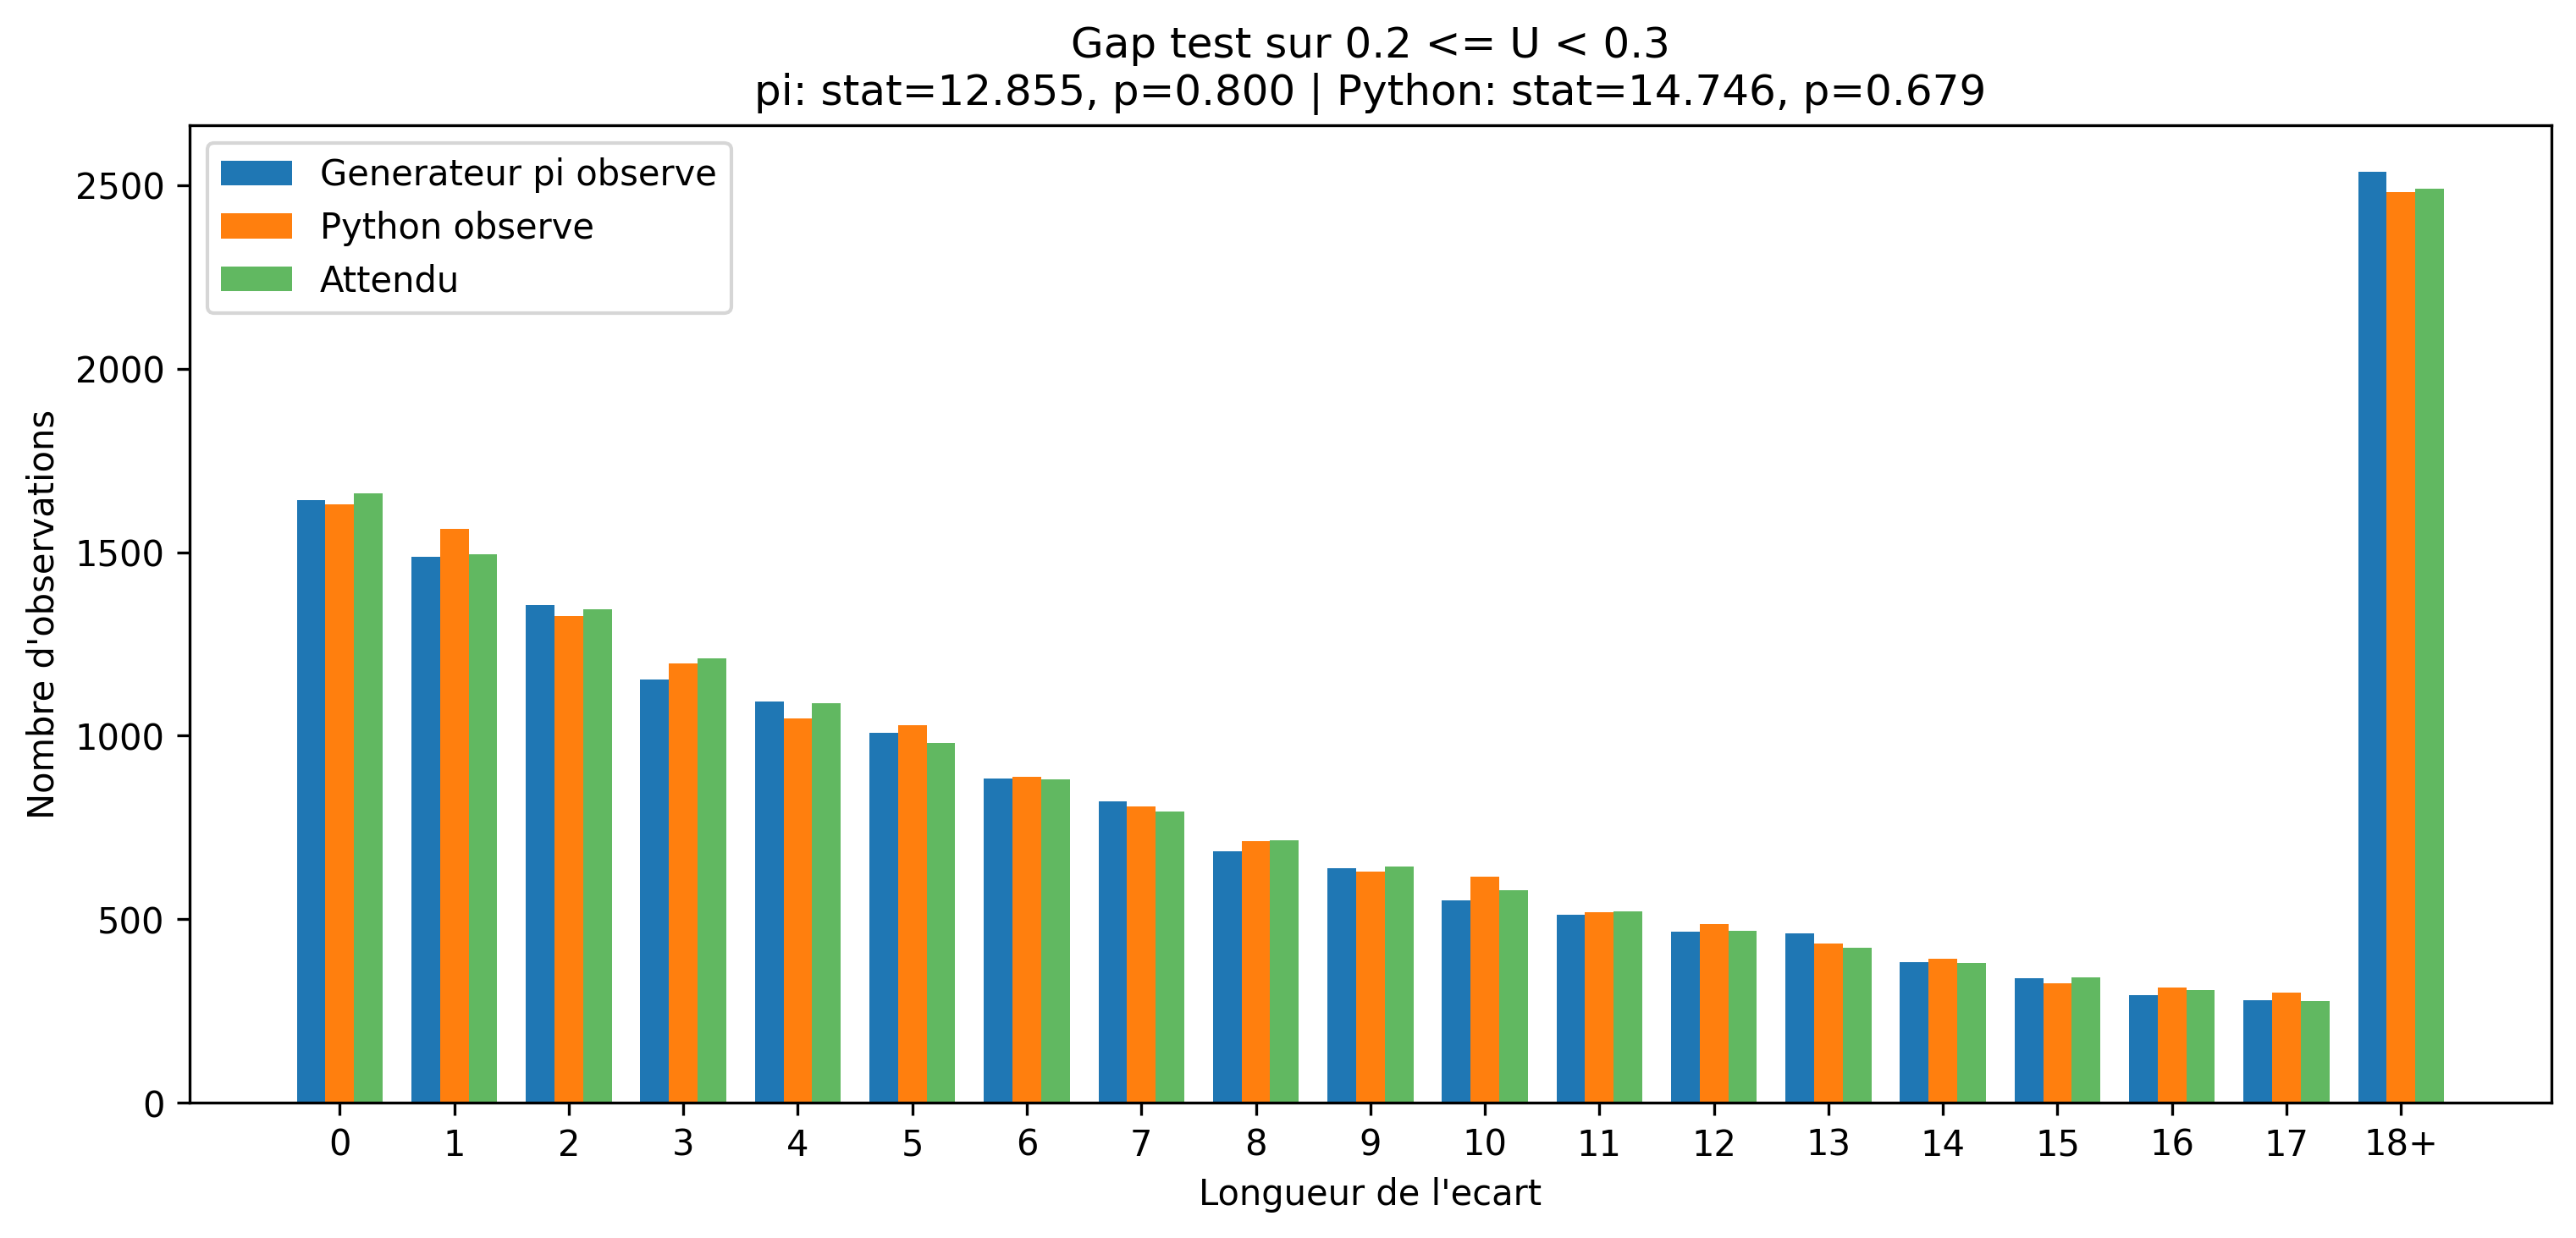
\includegraphics[width=0.9\textwidth]{comparison_gap_uniform.png}
\caption{Comparaison des deux générateurs par gap test sur l'événement $0{,}2 \leq U < 0{,}3$.}
\label{fig:comparison_gap}
\end{figure}

\section{Conclusion}

Les tests réalisés sur les décimales de $\pi$ donnent des résultats globalement compatibles avec une répartition uniforme des chiffres et avec le modèle attendu pour les écarts entre occurrences. Le test du $\chi^2$ sur les chiffres ne conduit pas à rejeter l'hypothèse d'uniformité. Le gap test met en évidence une p-value inférieure à $5\%$ pour le chiffre 4, mais ce résultat isolé doit être interprété dans le contexte de tests multiples et d'un échantillon très grand.

Le générateur construit à partir de $\pi$ est simple et explicite : il utilise des blocs non chevauchants de $k=6$ chiffres, transformés en entiers puis normalisés dans $[0,1[$. Pour ce choix de $k$, les tests du $\chi^2$, de Kolmogorov--Smirnov et du gap test donnent des résultats compatibles avec une loi uniforme. La comparaison avec \texttt{random.random()} montre des conclusions similaires sur l'échantillon étudié.

Ces expériences ne constituent pas une preuve de hasard véritable. Elles suggèrent seulement que, pour les tests et les tailles d'échantillon considérés, les décimales de $\pi$ et le générateur construit à partir de celles-ci présentent plusieurs comportements attendus d'une suite pseudo-aléatoire.

\end{document}
